%!TeX root=../Monografia - Mikhael Pinto.tex
%("dica" para o editor de texto: este arquivo é parte de um documento maior)

% Conteúdo da subseção sobre Usuários
% Este arquivo é importado em 02-implementacao.tex

Durante o piloto BikeSP, com
aproximadamente 1.200 participantes selecionados dentre 3.000 inscritos, a equipe de
suporte enfrentava demandas diárias de atendimento. Questões como ``não consigo acessar o aplicativo'', ``minha viagem não foi
computada'', ``como altero meu endereço cadastrado'' requeriam identificação rápida
do participante no sistema para diagnóstico e resolução. A interface de gerenciamento
de usuários tornou-se, portanto, o
ponto de partida no sistema administrativo  para praticamente todas as operações de suporte,
auditoria e análise.

A tela de usuários apresenta
tabela com seis colunas principais: ID (identificador único), nome
completo, email, CPF, número do Bilhete Único, e indicador mostrando se o participante
completou o cadastro de senha (permitindo acesso ao aplicativo). O sistema consulta dados pessoais vinculados aos cartões Bilhete Único ativos, utilizando técnicas de otimização para obter contagem total sem sobrecarregar o banco de dados --- importante para responsividade em conjuntos de dados com milhares de registros. A coluna ``Tem Senha'' verifica se existe senha cadastrada para aquele usuário, indicador crucial para diagnosticar
problemas de acesso (usuário inscrito mas sem senha configurada não consegue entrar no aplicativo).

O sistema oferece busca unificada por nome
(parcial, \textit{case-insensitive}\@) ou ID exato.
Por exemplo, buscar ``silva'' retorna ``Silva João'', ``Silvana Costa'', ``Marcos da
Silva'', enquanto buscar ``123'' retorna apenas o participante com ID exatamente 123.
Esta abordagem dual (nome parcial vs. ID exato) equilibra flexibilidade para buscas
exploratórias (quando administrador conhece apenas nome aproximado) e precisão para
operações dirigidas (quando ID já foi identificado em interação anterior ou viagem
específica). Importante notar que a busca não cobre email, CPF ou Bilhete
Único diretamente; para localizar por estes atributos, utiliza-se ordenação combinada com inspeção visual. A Figura~\ref{fig:usuarios_listagem} apresenta a interface de listagem (dados fictícios para fins ilustrativos).


\begin{figure}[htb]
    \centering
    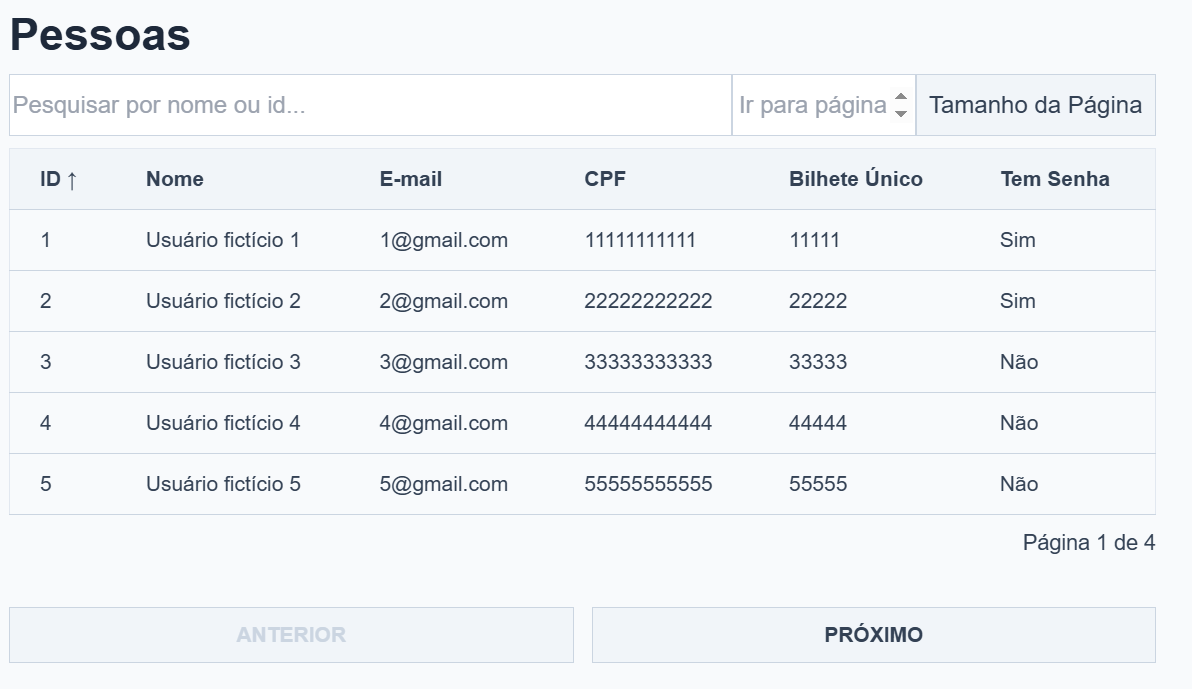
\includegraphics[width=0.95\textwidth]{figuras/pessoas.PNG}
    \caption{Interface de listagem de usuários com funcionalidades de busca, ordenação e paginação (dados fictícios).}
    \label{fig:usuarios_listagem}
  \end{figure}

Cada cabeçalho de coluna funciona como botão de
ordenação: primeiro clique ordena ascendentemente, segundo clique inverte para
descendente, com indicadores visuais (setas ↑↓) mostrando coluna ativa e direção.
Ordenação por nome facilita localização alfabética; por ID permite identificar
usuários cadastrados cronologicamente (IDs crescentes); por ``Tem Senha'' agrupa
participantes que completaram vs. não completaram ativação.

A interface oferece quatro densidades: 5, 10, 15
(padrão) ou 20 usuários por página, selecionáveis via dropdown. Navegação ocorre por
botões ``Anterior''/``Próximo'' (desabilitados nos extremos) ou campo de entrada
direta ``Ir para página X'', validando automaticamente se página solicitada existe.
Indicador ``Página X de Y'' fornece senso de escala do conjunto de dados. Esta
flexibilidade mostrou-se útil em diferentes contextos operacionais: densidade baixa
(5-10 itens) para inspeção cuidadosa com múltiplas abas abertas; densidade alta
(20 itens) para varredura rápida ou busca semi-manual quando termo de busca textual
não é aplicável.

A tela de usuários serve como ponto de
entrada para diversos fluxos operacionais críticos durante o piloto. \textit{Cenário
1: Suporte via email} --- participante reporta viagem não creditada; administrador
busca por nome, identifica ID, navega à tela de viagens filtrando por aquele ID,
localiza viagem em questão e diagnostica problema (ex: trajeto fora dos locais
cadastrados). \textit{Cenário 2: Problema de acesso ao app} --- participante não
consegue fazer login; administrador busca por nome, verifica coluna ``Tem Senha''; se
``Não'', orienta participante a completar cadastro via funcionalidade de redefinição
de senha. \textit{Cenário 3: Ajuste de localização} --- participante mudou de
endereço; administrador identifica ID, navega à tela de localizações, atualiza
coordenadas e endereço textual. \textit{Cenário 4: Contestação de viagem} ---
administrador recebe disputa; identifica usuário, obtém ID, acessa tela de
contestações para processar aprovação/rejeição. Em todos estes cenários, a rapidez
da busca e clareza da informação apresentada determinam eficiência do atendimento.

Durante o período de piloto, a
tela de usuários foi acessada diariamente pela equipe de suporte.
A métrica ``Tem Senha'' permitiu identificar participantes que não completaram ativação do aplicativo, 
orientando campanhas de engajamento. Recursos como ordenação e paginação reduziram significativamente a 
dependência de consultas manuais ao banco de dados, tornando as operações de suporte de primeiro nível mais ágeis
e acessíveis para toda a equipe.
